\documentclass{article}
% Thread: https://gemini.google.com/app/81401357ce6fbf66

\usepackage{amsmath}
\usepackage{amssymb}
\usepackage{graphicx}

\title{Nonsmooth Optimization via Quasi-Newton Methods}
\author{Scaffold}

\begin{document}

\maketitle

\section{Introduction}

Let $f: \mathbb{R}^n \rightarrow \mathbb{R}$
be a function we would like to minimize.
That is, we are interested in finding
$x^* = \arg\min_{x \in \mathbb{R}^n} f(x)$.
If $f$ is differentiable, the most straight-forward
method takes (small) steps in the direction
of steepest descent, i.e., the negative
gradient of $f$ at the current guess $x_k$.
This method, known as gradient descent is
often computationally attractive as the gradient
can be computed efficiently using automatic
differentiation tools.
However, gradient descent completely ignores
curvature information of $f$, which describes
how the gradient itself changes with respect
to the input $x$.
This can lead to slow convergence or additional
tuning of the step size.

The classical newton method aims to make informed
guesses of the best step size given the curvature
information of $f$.
Using the Taylor expansion of $f$ around $x_k$,
we can approximate $f$ as a quadratic function
and `jump' to the minimum of this approximation
in the next step.
In general, the next guess $x_{k+1}$ is given by:
\begin{equation}
    x_{k+1} = x_k - (\nabla^2 f(x_k))^{-1} \nabla f(x_k),
\end{equation}
where $\nabla f(x_k)$ is the gradient of $f$ at $x_k$
and $\nabla^2 f(x_k)$ is the Hessian matrix of $f$ at $x_k$.
The algorithm requires the Hessian matrix to always be invertible.
This may not be the case if $f$ has a point of zero
curvature.
In some cases, it can also be computationally expensive
to compute the (inverse) Hessian matrix.

\section{Quasi-Newton Methods}

In quasi-newton methods, we approximate the Hessian
matrix $\nabla^2 f(x_k)$ by a matrix $B_k$.
This approximation is done by inspecting how the
gradient changes between two consecutive steps.
One example is the Broyden-Fletcher-Goldfarb-Shanno (BFGS)
algorithm, which directly approximates the inverse
Hessian matrix saving us the need to solve a linear
system in each iteration.
We will not be looking at the details of the BFGS
algorithm, so we shall focus on the general idea
and investigate why it works for non-smooth problems.

In a non-optimized form~\footnote{
    that is, without the direct approximation of the
    inverse Hessian as mentioned above
}, the BFGS algorithm can be
summarized as follows. At each iteration $k$, the algorithm
% https://en.wikipedia.org/wiki/Broyden%E2%80%93Fletcher%E2%80%93Goldfarb%E2%80%93Shanno_algorithm#:~:text=.-,Algorithm,-%5Bedit%5D
\begin{enumerate}
    \item computes the gradient $\nabla f(x_k)$,
    \item solves the linear system $B_k p_k = -\nabla f(x_k)$
          to obtain search direction $p_k$,
    \item performs a one-dimensional line search over
          $f(x_k + t s_k)$ to find a suitable step size $t$,
    \item sets $s_k = t p_k$, updates $x_k \leftarrow x_k + s_k$, and
    \item computes $y_k = \nabla f(x_{k+1}) - \nabla f(x_k)$ to update
          \[
              B_{k+1} = B_k + \frac{y_k y_k^T}{y_k^T s_k}
              - \frac{B_k s_k s_k^T B_k}{s_k^T B_k s_k}.
          \]
\end{enumerate}
Convergence is typically `reached' when the norm of the gradient
$\| \nabla f(x_k) \| < \epsilon$ becomes less than some
small tolerance $\epsilon$.
It is known that for smooth functions, quasi-Newton methods
like the BFGS algorithm work well and converge quickly.

\section{Nonsmooth Problems}

\begin{itemize}
    \item Defining Armijo-Wolfe conditions
          \begin{quote}
              ``Given constants $c_1 < c_2$ in the interval $(0, 1)$, we
              seek an Armijo-Wolfe step, which we define to be a number
              $t > 0$ satisfying the Armijo and Wolfe conditions \dots'' [cite: 174]
          \end{quote}

          % Transition: Briefly explain the line search algorithm and its properties.
\end{itemize}

Often, real-world optimization problems are non-smooth, for example
if the objective function contains absolute values or maxima.
Gradient descent methods can end up oscillating around the minimum
as the derivative must not smoothly change but can jump.

\begin{figure}
    \centering
    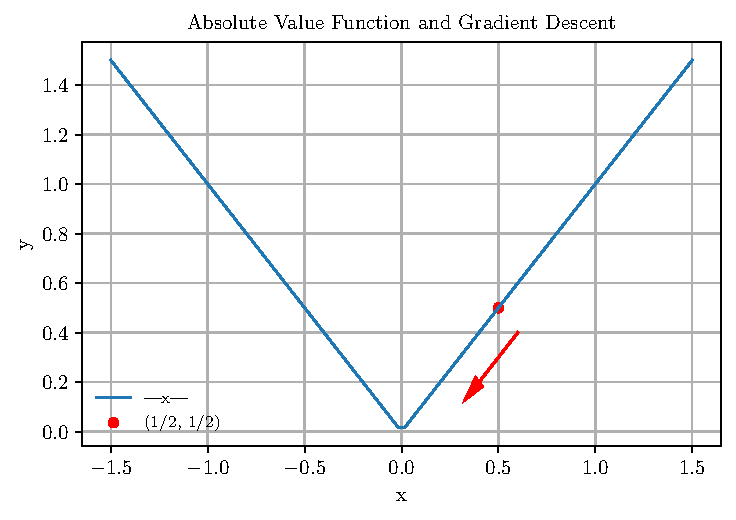
\includegraphics[width=0.7\textwidth]{plots/abs_val_func.pdf}
    \caption{The absolute value function and Gradient Descent.}
    \label{fig:abs_value_function}
\end{figure}

As we can see in Figure~\ref{fig:abs_value_function}, with a step
size of $1$, gradient descent would jump to from $x=1/2$ to $x=-1/2$,
and then back to $x=1/2$ and oscillate indefinitely.

\section{Example: The Absolute Value Function}

To illustrate the behavior of
quasi-Newton methods with an inexact
line search for non-smooth functions,
consider the absolute value function,
$f(x) = |x|$. This function is
non-differentiable at $x = 0$, posing a
challenge for traditional optimization
methods.
% What happens to gradient descent here?
% Illustrate with some iterations by hand

Theoretical analysis shows that
quasi-Newton methods with an appropriate
inexact line search exhibit R-linear
convergence with a rate of
$\frac{1}{2}$ for the absolute value
function. This indicates that the
method makes consistent progress towards
the minimum, even in the presence of
non-differentiability.

\section{Code Example: Minimizing the L1 Norm}

% Insert code example and explanation here.

\section{Applications}

\begin{itemize}
    \item Briefly mention applications like condition geodesic problems and
          shape optimization.
\end{itemize}

\section{Conclusion}

% Summarize the key findings and contributions of the paper.

\end{document}